\documentclass[prc,superscriptaddress,showpacs,floatfix]{revtex4}
\usepackage[dvips]{graphicx}
\usepackage{epsfig}
\usepackage{pst-plot}
\usepackage{bm}
\usepackage{bbm}
\usepackage{mathrsfs}
\usepackage{amsfonts}
\usepackage{amssymb}
\usepackage{lscape}

\begin{document}

\title{Coupled-Cluster calculation of the $^{3-5}$He 
  isotopes with Gamow-Hartree-Fock basis}
\author{G.~Hagen}
\affiliation{Physics Division, Oak Ridge National Laboratory, P.O. Box 2008, Oak Ridge, TN 37831, U.S.A.}  
\affiliation{Department of Physics and Astronomy, University of Tennessee, 
  Knoxville, Tennessee 37996, U.S.A.}
\author{D.J.~Dean}
\affiliation{Physics Division, Oak Ridge National Laboratory, P.O. Box 2008, Oak Ridge, TN 37831, U.S.A.}  
\author{M.~Hjorth-Jensen}
\affiliation{Department of Physics and Center of Mathematics for Applications, 
University of Oslo, N-0316 Oslo, Norway}
\author{T.~Papenbrock}
\affiliation{Department of Physics and Astronomy, University of Tennessee, 
  Knoxville, Tennessee 37996, U.S.A.}
\affiliation{Physics Division, Oak Ridge National Laboratory, P.O. Box 2008, Oak Ridge, TN 37831, U.S.A.}  


\date{\today}
\begin{abstract}
We present \emph{ab-initio} CCSD calculations 
of the $^{3-5}$He ground states. 
We perform these calculations using a mixed basis 
of oscillator- and complex Woods-Saxon
states for chosen partial waves. From this starting point we 
build a spherical Gamow-Hartree-Fock basis
from a renormalized interaction of the low-momentum type generated 
from the  N$^3$LO two-body potential.
The Gamow-Hartree-Fock basis, which is a Berggren basis,
treats bound, resonant and continuum states on an
equal footing, and is therefore optimal for the 
description of nuclear states which may be embedded in 
the continuum. Within this \emph{ab-initio} 
approach we are able to calculate that $^{3-4}$He are stable 
against particle decay, while $^5$He 
has a non-neglible width and is therefore unstable with 
respect to one neutron emission, as is the case experimentally. 
We illustrate from these calculations that the CCSD
approach is as accurate for closed shell nuclei 
as for open shell nuclei with $\pm 1$ nucleon outside  a closed shell. 
Finally, we perform various tests on the convergence of 
our CCSD results.  We find that our results are well converged 
with respect to basis size and discretization of the continuum integral 
defining our Berggren basis.
\end{abstract}
\pacs{21.60.Cs, 21.10.-k, 24.10.Cn, 24.30.Gd}
\maketitle

\section{Introduction}
In nuclear physics one would ideally like to 
start from nucleon degrees of freedom.
The dominant philosophy within the nuclear theory community is 
that the nucleus (at low energies) 
as a whole  may be fully described in terms of the 
the interactions between these constituents.
\emph{ab-initio} methods such as the Green's
Function Monte Carlo (GFMC) approach 
\cite{pieper1,pieper2,pieper3,pieper4,pieper5,pieper6}, 
and the large-basis no-core Shell Model 
(NCSM) approach \cite{bruce1,bruce2,bruce3,bruce4}
have been successfully applied to the 
description of light nuclei. However, both 
approaches have limitations with respect to basis 
size and the number of active
nucleons in the systems. More importantly, these 
methods have not been utilized to investigate nuclear
widths in unstable nuclei. 

It is well known that quantum systems with a 
tendency to decay by emission of fragments 
cannot be described as closed quantum systems, 
in which particles are trapped in an infinite well 
such as a harmonic oscillator. In exotic nuclei near the 
driplines the outermost nucleons are mainly occupying 
loosely bound or unbound single-particle orbitals, 
resulting in matter densities with halo characteristics. Such 
matter densities cannot 
easily be described by the use oscillator 
functions which do not display the correct asymptotic behaviour.  
A proper description of loosely bound and unbound 
nuclei should take into account the coupling of 
the internal with the external 
environment.  The coupling of the 'external' continuum of 
positive energy states, with the 'internal' nuclear states has 
for a long time been a basic ingredient in nuclear reaction theory. 
Feshbach was the first to formulate a unified 
description of direct and compound nuclear reactions within 
the projection operator method \cite{feshbach1,feshbach2}. �
He showed that the coupling of the internal with the 
external environments could 
give rise to compound nuclear states, such as 
multi-channel resonances. Also, in atomic physics Feshbach resonances
are of great importance. In the early 60's, at the same time as
Feshbach's work, Fano \cite{fano} 
discussed how the mixing of a configuration 
belonging to a discrete spectrum with configurations 
belonging to a continuous spectrum
gives rise to the phenomena of 
\emph{autoionization}, which is considered a 
multi-channel 
resonance. 

In nuclear physics, the Gamow shell model 
\cite{michel1, michel2, michel3, witek1, witek2, 
roberto, betan, betan2,hagen1, hagen2}
has proven to be a reliable tool in the description 
of nuclei where continuum aspects
play a dominant role. The basic idea in the Gamow shell 
model approach is to construct 
a many-body basis from a generalized single-particle 
basis which treats bound, resonant and continuum states 
on equal footing. Berggren was the first to rigorously 
derive such a basis \cite{berggren}. 
The Berggren basis is an analytic continuation 
of the usual completeness relation in the complex energy plane. 
Recently, we reported the first results on loosely bound and resonant 
states in nuclei, starting from a realistic interaction and a Gamow - Hartree - Fock basis \cite{hagen3}. 
However, an \emph{ab-initio} description of such nuclei within the Gamow shell model approach 
might presently not be feasible since the computational cost scales combinatorially with 
the number of orbitals, and one typically needs a large number of orbitals for each partial 
wave in order to discretize the continuum integrals accurately.

In order to be able to provide an \emph{ab-initio} description of 
nuclei with loosely bound and unbound characteristics we may need
to depart from standard matrix diagonaliztion methods. 
In this work we discuss the \emph{coupled-cluster} 
method ~\cite{coester,coesterkummel,cizek,palduscizek,cc1,cc2,cc3,cc4} 
as a starting point for the description of 
exotic nuclei. Computational scaling of the coupled-cluster method
enables one to reach accurate results in extremely large model 
spaces. At the coupled-clusters in singles and doubles (CCSD) 
level, floating-point 
operation counts scale as $n_o^2n_u^4$, where $n_0$ is the number
of occupied orbitals and $n_u$ is the number of unoccupied 
orbitals in the single-particle basis.  Such soft scaling 
when compared to the nearly combinatorial scaling of diagonalization 
procedures (as a function of basis size and/or particle number) allows 
one to build an extension of \emph{ab-initio} 
descriptions of nuclei to the medium mass region starting 
with nucleon degrees of freedom. 
The coupled-cluster method is also capable of 
systematic improvements and amenable to parallel computing. 

The outline of this paper is as 
follows. In Sec.~\ref{sec:cc} we give a brief outline of the
coupled-cluster theory. In Sec.~\ref{sec:renorm} it is discussed 
how one may derive a renormalized interaction of the low-momentum type ($V_{low-k}$) from 
similarity transformation techniques. In Sec.~\ref{sec:ghf} it is outlined how 
a Gamow-Hartree-Fock basis may be derived from the bare nucleon-nucleon interaction, and in
Sec.~\ref{sec:results} we present CCSD results of 
the ground states of the 
$^{3-5}$He isotopes using a Gamow-Hartree-Fock basis. 
Convergence with respect to basis size and 
number of discretization points is also analysed. 
Finally, in Sec.~\ref{sec:conc} we conclude 
and mention future perspectives for this work. 

\section{Coupled-Cluster Theory}
\label{sec:cc}
In coupled cluster theory we make an exponential ansatz for the exact correlated 
ground-state expressed through, 
\begin{equation}
\hat H \vert \Psi \rangle  = \hat H \exp(T) \vert \Phi_0 \rangle = E \exp(T) \vert \Phi_0 \rangle,
\label{eq:cc1}
\end{equation}
here $\vert \Phi_0 \rangle$ is a chosen non-correlated reference Slater-determinant such as for 
example the Hartree-Fock state. The fully correlated 
many-body state $\mid\Psi\rangle$ is constructed by 
letting the correlation operator $\exp(T) $  operate on $ \Phi_0$. 
The operator $T$ is a linear combination of 
$n$-particle-$n$hole excitation operators $T = T_1 + T_2 + ...$ of the form,
\begin{equation}
T_n = \sum_{ab...,ij...}t_{ij...}^{ab...}a_a^\dagger a_b^\dagger \cdot\cdot\cdot a_j a_i.
\end{equation}
In order to derive the coupled-cluster equations we start by rewriting
the Hamiltonian in normal-ordered form,
\begin{equation}
  H = \sum_{pq} f_{pq}\left\{ a_p^\dagger a_q\right\} + {1\over 4}\sum_{pqrs} \langle pq \vert \vert rs \rangle 
\left\{ a_p^\dagger a_q^\dagger  a_s a_r \right\} + \langle \Phi_0 \vert H \vert \Phi_0 \rangle = 
H_N  + E_0,
\end{equation}
here $H_N$ is the normal ordered part of $H$ and $E_0$ is just the vacuum expectation value of $H$. 
The Fock matrix element $f_{pq}$ is given by, 
\begin{equation}
  f_{pq} = \langle p\vert t \vert q \rangle + \sum_i \langle pi \vert \vert ri \rangle.
\end{equation}
Using the normal ordered Hamiltonian and projecting Eq.~(\ref{eq:cc1}) from the left 
with $\langle \Phi_0\vert \exp(-T)$ gives an equation for the coupled cluster correlation energy, 
\begin{equation}
  E_{\mathrm{CC}} = \langle \Phi_0 \vert \exp(-T) \hat H_N \exp(T) \vert \Phi_0 \rangle.
\end{equation}
This equation may be simplified by using the Hausdorff commutator expansion of the similarity transformed
Hamiltonian $ \exp(-T) \hat H_N \exp(T) $, which truncates exactly at quadruply nested commutators 
for a two-body Hamiltonian. Using Wick's theorem for the commutators it may be shown that the only 
nonzero terms in the Hausdorff expansion are those in which $H_N$ has at least one contraction with 
every cluster operator on its right, which is expressed through, 
\begin{equation}
  \exp(-T) \hat H_N \exp(T) \vert \Phi_0 \rangle = \left[ H_N \exp(T) \right]_C \vert \Phi_0 \rangle.
\end{equation}
here $C$ indicates terms in which the Hamiltonian is connected to 
every cluster operator on its right.
The equation for the Coupled-Cluser energy is then simply given by,
\begin{equation}
  \nonumber
  E_{\mathrm{CC}} = \langle \Phi_0 \vert \left[ H_NT_1 + {1\over 2}H_NT_2  + {1\over 2}H_NT_1^2 \right]_C \vert \Phi_0 \rangle = 
  \sum_{ia}f_{ia}t_i^a + {1 \over 4}\sum_{abij} \langle ij\vert \vert ab\rangle t_{ij}^{ab} + 
  {1\over 2}\sum_{ijab} \langle ij\vert \vert ab\rangle t_i^a t_j^b.
  \label{eq:cc2}
\end{equation}
This equation for the coupled-cluster correlation energy is an exact result which holds for two-body Hamiltonians and 
is independent of any truncations of the correlation operator $T$. In order to evaluate the coupled-cluster 
correlation energy it is obvious that we need to determine the $1p-1h$ and $2p-2h$ excitation amplitudes,
$t_i^a$ and $t_{ij}^{ab}$, appearing in Eq. ~(\ref{eq:cc2}).
Although only $t_i^a$ and $t_{ij}^{ab}$ 
amplitudes appear in the energy expression in Eq.~(\ref{eq:cc2}), the higher order cluster equations 
will modify the equations for $t_i^a$ and $t_{ij}^{ab}$  and 
therefore indirectly the coupled cluster 
energy equation.
The algebraic equation for the excitation amplitudes $t_{ij...}^{ab...}$ are obtained by left-projecting 
the similiarity transformed Hamiltonian with an $n$-particle-$n$hole excited Slater determinant giving
\begin{equation}
\langle \Phi_{ij...}^{ab...} \vert \left[ H_N \exp(T) \right]_C \vert \Phi_0 \rangle = 0,
\end{equation}
When written in its full glory one ends up with a 
non-linear set of equations for the excitation amplitudes. The derivation of the amplitude equations is
a tedious task using Wick's theorem, but using a diagrammatic technique the amplitude and energy equations may 
be written down much more easily.  The amplitude equations are nonlinear, and  may be solved iteratively 
using convergence accelerators such as the direct inversion in the iterative subspace (DIIS) \cite{diis} 
technique or Krylov subspace accelerated inexact Newton (KAIN) techniques \cite{kain}. 
In our coupled-cluster calculations of open-shell nuclei we have found that convergence is 
considerably much more difficult to obtain than for closed shell nuclei. However, combining 
the iterative convergence accelerators with step-restriction and line-search in each iteration, 
convergence can be obtained within a reasonable number of iterations.
Approximations in coupled-cluster theory appear only when the linear series is truncated at a level $T_n$,
where $n$ is smaller than the number of particles in the system, and 
in this work we report results for the 
$^{3-5}$He isotopes truncating the correlation operator $T$ at 
the CCSD level. 
We note that
even though the $T$-operator is truncated at the $2p-2h$ level, the exponential ansatz indirectly 
induces higher excitations since we have products of $T_1 $ and $T_2$ operators, 
when expanding the exponential.  

\section{Renormalized nucleon-nucleon interaction of the low-momentum type.}
\label{sec:renorm}
The nuclear many-body Hamiltonian we work with is given by,
\begin{equation}
H = T - T_{\mathrm{CoM}} = \left( 1 - {1\over A}\right) \sum_{i=1}^A 
  { {\bf k}_i^2\over 2m } +  \sum_{i<j}^A \left (V(i,j)-\frac{{\bf k}_i \cdot {\bf k}_j}{mA}\right), 
\end{equation} 
here $ V $ is the nucleon-nucleon interaction given by the N$^3$LO 
effective field theory expansion \cite{n3lo1}, based 
on chiral perturbation theory next-to-next-to-next-to-leading order.  
One would need huge basis sets in order to capture the 
high momentum modes of the interaction and achieve convergence for 
energies and wave functions. In order to make calculation feasible, the nucleon-nucleon interaction
has to be renormalized in order to soften the core of the 
interaction. In this work we
construct a renormalized interaction following the scheme 
outlined in 
\cite{vlowk,suzuki4,suzuki5,bogner,nogga}. 
We construct an effective interaction 
where the high momentum modes 
of the full two-body interaction have been integrated out. 
This interaction has become known as
$V_{\mathrm{low-k}}$, which is energy and nucleus 
independent, and reproduces exactly 
nucleon-nucleon scattering data below a cutoff $\Lambda$, which determines the 
border between low and high momentum modes.  

In the following  we briefly outline how to obtain a Hermitian 
interaction $V_{\mathrm{low-k}}$ based on the
similarity transformation discussed in Refs.~\cite{suzuki2,suzuki3,suzuki4,suzuki5}. 
A unitary transformation can be parametrized in terms of the model space $P$ and the excluded
space $Q$ via 
 \begin{equation}
 U = \left( \begin{array}{cc} P (1 + \omega ^\dagger \omega  )^{- 1/2} P & - P
 \omega ^\dagger ( 1 + \omega \omega ^\dagger )^{- 1/2}  Q \\
 Q \omega  ( 1 + \omega ^\dagger \omega  )^{- 1/2} P
 & Q (1 +  \omega \omega ^\dagger )^{- 1/2} Q
 \end{array} \right),
 \end{equation}
where the wave operator $\omega$ is defined to satisfy the condition
\begin{equation} 
\label{eq:decoup}
\omega  = Q \omega  P,
\end{equation}
 the so-called decoupling condition \cite{okubo}.
 Note that the unitary transformation 
 is by no means unique. In fact, one can construct infinitely many different 
 unitary transformations
 which decouple the $P$ and the $Q$ subspaces, as discussed by Kuo {\em et al} \cite{tom2004}.
The above transformation  
 depends only on the operator $\omega$ which mixes the $P$ and $Q$
 subspaces and is in some sense ``the minimal possible'' 
 unitary transformation. 
 Following the method of Ref.~\cite{suzuki4}, one obtains
 \begin{equation}
 U=(1+\omega-\omega ^{\dagger})
 (1+\omega \omega ^{\dagger} +\omega ^{\dagger}\omega )^{-1/2}.
 \end{equation}
 The operator $U$ leads to the effective interaction $\tilde{V}$ using the definition
 \begin{equation}
 \label{eq:V_eff}
 \tilde{V}=U^{-1}(T+V)U-T,
 \end{equation}
 where $T$ is the kinetic energy of the nucleons 
and $V$ is the free nucleon-nucleon interaction. If we can determine the wave operator $\omega $ 
the spectrum of the effective Hamiltonian  will correspond to exactly $N_P$ 
eigenvalues of the full problem.  In order to derive the 
renormalized interaction in momentum space, 
one starts with the following definitions of the $P-$ and $Q-$space, 
\begin{equation}
  P = \left\{ \vert \bar{k}\rangle, \:\: \vert k\vert  \leq \Lambda \right\}, \:\:
  Q = \left\{ \vert \bar{k}\rangle, \:\: \Lambda < \vert k\vert < \infty \right\}.
\end{equation}
The model space $P$ here defines all the low-momenutm modes determined by the cutoff $\lambda$, while
the complement $Q-$ space consists of the high-momentum modes. Solving the momentum space
Schr\"odinger equation in the full space, one may obtain the solution of the wave-operator $\omega$ in a
plane-wave basis and finally obtain the effective low-momentum interaction $V_{\mathrm{low-k}}$,
\begin{eqnarray}
  \nonumber \langle \bar{k}\vert P V_{\mathrm{low-k}} P\vert \bar{k}'\rangle & = & 
  \sum_{k''}\sum_{k'''}
  \langle \bar{k}\vert P(P+\omega^{\mathrm{T}}\omega )^{1/2} P\vert \bar{k}'' \rangle
  \langle \bar{k}''\vert P(T+V)P \vert \bar{k}'''\rangle 
  \langle \bar{k}'''\vert  P(P+\omega^{\mathrm{T}}\omega )^{-1/2}P \vert \bar{k}'\rangle \\
  & - & {k^2\over m} \delta_{kk'},
\end{eqnarray} 
where $ \vert \bar{k} \rangle�= k\sqrt{w}�\vert k \rangle $.
See Ref.~\cite{suzuki4} for further details.  
Typically $\Lambda $ is chosen around 2~$\mathrm{fm}^{-1}$,  in
order to capture the physics of elastic nucleon-nucleon scattering 
for energies $ < 350 $ MeV. 
However, the construction 
of an effective two-body interaction in a model-space for the $A-$body problem will necessarily generate 
three- and many-body forces. At the two-body level it has been shown that all low-momentum 
interactions collapse onto the same curve for a cutoff 
$\sim 2$~$\mathrm{fm}^{-1}$, and therefore displays
a model-independence. This is only true at the two-body level. 
Many-body calculations starting with a two-body low-momentum 
interaction display a considerable dependence on
the particular interaction model from which it 
was derived. Further, many-body 
calculations starting with a two-body low-momentum 
interaction typically gives rise to considerable
cutoff dependence and over-binding, 
especially in the medium mass regimes. 
The model-independence can only be 
restored at the $A$-body level by introducing all $A-$ body 
effective interactions generated through a similarity transformation 
of the $A$-body problem. 
The hope is that three-body effective interactions are 
sufficient to restore model-independence, 
and that they can be treated perturbatively. Preliminary CCSD
results for the ground state of $^{16}$O indicates that the low-momentum three-body force is indeed 
repulsive and can be treated perturbatively \cite{papenbrock}. 
However, in this work we have truncated the Hamiltonian at the two-body level and neglect 
the effect of three-body forces. For all results reported in this work we constructed our 
low-momentum interaction from the N$^3$LO potential 
at a cutoff of $\Lambda=2$~fm$^{-1}$.

\section{Gamow-Hartree-Fock single-particle basis}
\label{sec:ghf}
In our study of $^5$He which is an unbound nucleus, 
the single-particle basis has to be constructed in such a way that 
correlation effects between nucleons in the scattering continuum can take place. 
To account for this non-neglible coupling with the continuum, we construct 
our basis using the Berggren formalism \cite{berggren} in which bound, resonant and continuum states
are treated on an equal footing. This single-particle
basis is therefore optimal for construction 
of a many-body basis in which loosely bound and unbound nuclear states may be expanded.
For our study of the $^{3-4}$He ground states a Berggren representation is not
necessary since they are stable nuclei. However, we use 
the same Berggren basis for all nuclei studied here, so that we may be able to 
confirm the stability of $^{3-4}$He and the resonant character 
of $^5$He.

Further, we would like to construct our single-particle basis from the self-energy 
of the nucleon-nucleon interaction so that our basis is optimal for the particular nucleus under study. 
At lowest order in perturbation theory, the self-energy is just the Hartree-Fock basis. 
In order to construct the Hartree-Fock basis one needs to transform the
nucleon-nucleon interaction from the 
relative and center of mass frame to the laboratory frame. 
In the case of an oscillator basis this procedes through the well-known Moshinsky transformation, for general bases
the transformation is carried out with the so-called vector 
brackets \cite{balian69,wc72,kkr79,bonatos}.
If our basis is defined in the complex energy plane, the vector-bracket transformation coefficients have 
to be analytically continued in the complex plane. 
However, the vector-bracket transformation coefficients are not easily continued in the complex $k$-plane, 
and we therefore procede via the numerically and mathematically simpler route outlined in Ref.~\cite{hagen3}. 
In Ref.~\cite{hagen3} it was also illustrated how matrix elements 
of the nucleon-nucleon interaction may be obtained in a Berggren basis 
by expanding the interaction 
in a finite oscillator basis, i.e.   
\begin{equation}
  \langle ab \vert V_{\mathrm{osc}} \vert cd \rangle \approx \sum_{\alpha \leq \beta}^N \sum_{\gamma \leq \delta}^N 
  \langle ab \vert \alpha \beta\rangle \langle \alpha\beta \vert  V_{\mathrm{low-k}} \vert \gamma \delta \rangle 
  \langle \gamma \delta \vert c d \rangle, 
  \label{eq:nn_lab_approx}
\end{equation}
where the two-body oscillator completeness has been truncated at $N$ for numerical purposes.
Using a renormalized interaction of the low-momentum type, 
energies and wave functions of loosely bound and resonant systems 
were  shown to converge quickly with respect to the 
oscillator basis size. The fast convergence is 
just another illustration of the fact that renormalized interactions reduce infinite spaces to smaller model spaces, 
making calculations practical. 
From the matrix elements in Eq.~(\ref{eq:nn_lab_approx}), we may construct our Gamow-Hartree-Fock basis from 
\begin{equation}
  \langle a \vert h_{\mathrm{HF}} \vert c \rangle = \langle a \vert  t \vert c \rangle + 
  \frac{1}{\hat{j_{a}}^2} \sum_{J}\sum_{h}\hat{J}^2 \langle ah \vert V_{\mathrm{osc}} \vert ch \rangle,
\end{equation}
where $h$ labels all quantum number of the proton and neutron hole states,
and $\hat{J}^2=J(J+1)$. The Hartree-Fock equation 
is iterated until self-consistency is obtained.
One typically needs  single-particle orbits comprising the $f$ and $g$ shells 
in no-core calculations, in addition to  including 
the continuum for each partial wave $l$. 
Therefore we are performing our calculations in an enormous many-body configuration space 
due to the dense discretization of the continuum integral,  
and even CCSD calculations become extremely 
computationally memory and time consuming.

To make calculations numerically feasible at present we therefore initialize
our Hartree-Fock calculations with a mixed basis consisting of a finite set of 
Complex Woods-Saxon bound, resonant and non-resonant continuum states and a finite set of
Harmonic Oscillator basis states for chosen partial waves. 
For  protons we strictly 
define the space by a finite set of harmonic oscillator wave functions, while 
for the neutron space we use a complex 
Woods-Saxon basis for the $s-p$ partial waves and 
harmonic oscillator wave functions for the higher partial waves $d-g$.
This choice of mixed basis may be 
justified since we are dealing with the 
ground states of the $^{3-5}$He isotopes.
For these nuclei the proton separation energy
is typically at the order of $20-30$~MeV and 
they are mainly occupying deeply bound $s$-orbits.
On the other hand it is well known that the $^5$He 
ground state is a resonance with width $\sim 0.65$MeV and 
with spin and parity $J^\pi = {3/2}^-$, implying that the outermost neutron 
in $^5$He is mainly in the $p_{3/2}$ shell. 

We construct the complex Woods-Saxon basis by employing the 
Contour Deformation Method in momentum space, as
outlined in Ref.~\cite{hagen1}. In 
order to check the validity and convergence of our results,
we construct our single-particle Berggren basis 
on two very different contours in the complex $k$-plane. 
In Figs.~\ref{fig:contour1} and \ref{fig:contour2} we sketch how 
the two different contours $L_1^+$ and 
$L_2^+$ are defined respectively. The contour 
\ref{fig:contour1} is of triangular shape and defined by 
three line segments joined by the points $A$ and $B$ in the complex $k$-plane.
The contour $L_2^+$ consists of a rotated and a 
translated line segment joined at the
point $A$  in the complex $k$-plane. Utilizing a contour 
of the type $L_2^+$, it was shown in Ref.~\cite{hagen1} 
that both resonant and anti-bound states converge quickly 
with respect to the number of integration points. 
Further it was shown that for the contour $L^+_2$, stable solutions of all physical 
scattering amplitudes, such as the $t$-matrix, may be obtained by a spectral representation of the Green's function.
We discretize the contours $L_1^+$ and $L_2^+$ by 
Gauss-Legendre quadrature.  

\begin{figure}
  \resizebox{8cm}{5cm}{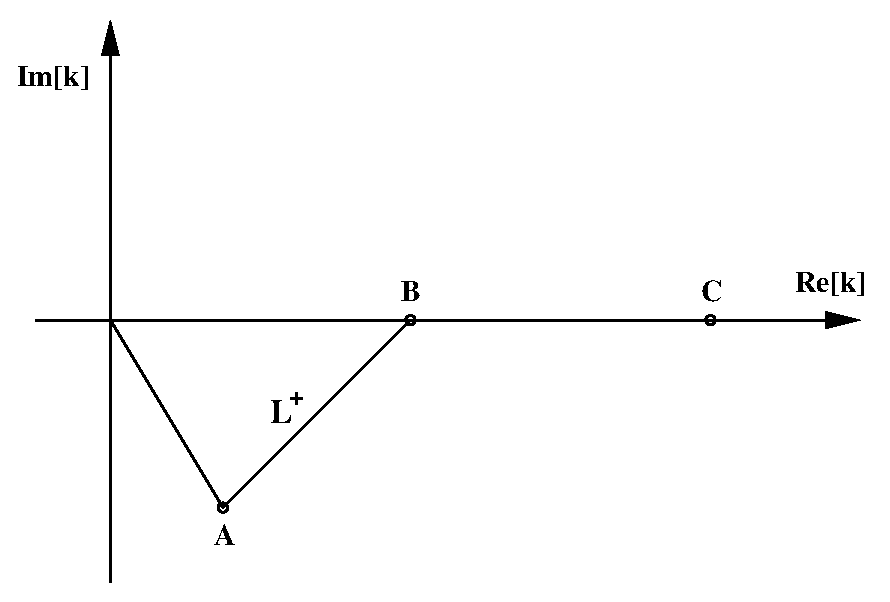
\epsfig{file=fig1.eps}}
   \caption{Contour $L^+_1$ in the complex $k$-plane 
     used in construction of the single-particle Berggren basis. 
     The contour in specified by the points $A,B$ and $C$ discussed in the text.}
\label{fig:contour1}�
\end{figure}

\begin{figure}
  \resizebox{8cm}{5cm}{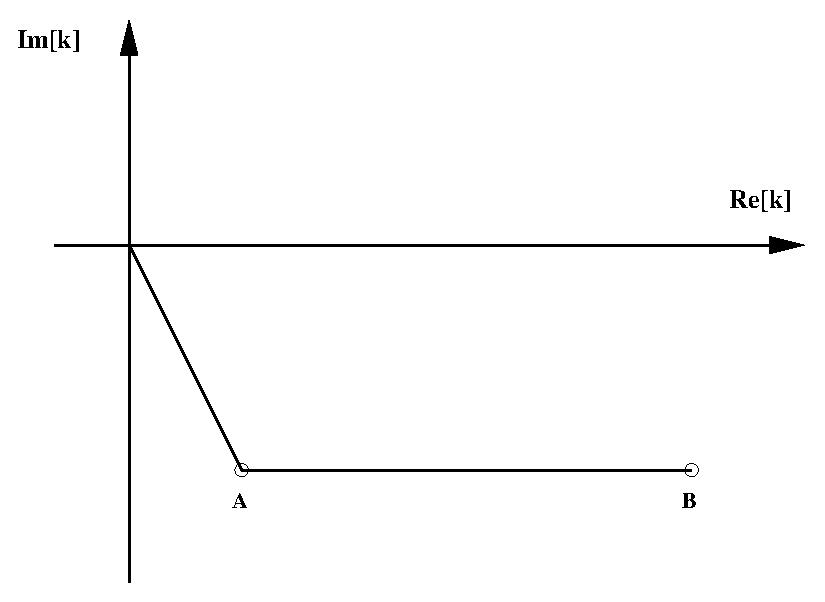
\epsfig{file=fig2.eps}}
   \caption{Contour $L^+_2$ in the complex $k$-plane 
     used in construction of the single-particle Berggren basis. 
     The contour in specified by the points $A$ and $B$ discussed in the text.}
\label{fig:contour2}�
\end{figure} 
Ideally we would like to construct our many-body Berggren basis utilizing 
as few continuum states as possible.
In Tabs.~\ref{tab:n3lo_sp_he5_1} and ~\ref{tab:n3lo_sp_he5_2}  
we study the convergence of the  $s_{1/2}�$ hole and $p_{3/2}$ particle
states in $^4$He at the Hartree-Fock level with respect to number of integration points, using 
the two contours given in Figs.~\ref{fig:contour1}�and \ref{fig:contour2}. 
The total number of integration points is given by $n$, while $n_i$ gives the number 
of points used to discretize a given line segment on the contour. 
The $L_1^+$ contour is defined by the points $A = 1.5 - 2i$MeV and $ B = 3$MeV, and the 
contour $L_2^+$ by the point $A = -2i$MeV in the complex energy plane. The corresponding 
points in the complex $k$-plane are proportional to the square root of the points in the 
energy plane. 
We see that the hole and particle 
energies converge to the same values for the two different contours; 
this is expected since 
the location of  bound- and resonant poles in the complex $k$-plane is given by the pole structure of 
the $S$-matrix and not by the particular choice of contour. Further, we see that satisfactory 
convergence is obtained with a total number of points given by $n \sim 20$. For the proton space
we used $5s5p$ oscillator  wave functions with $\hbar \omega =20$MeV. The $p_{3/2}$ proton state does not
have a width, this is a consequence of using harmonic oscillator functions for our proton-space.
 \begin{table}[htbp]
  \caption{Convergence of the $s_{1/2}$ hole and the $p_{3/2}$ particle states in 
    $^4$He with increasing number of discretization points along the triangular contour $L^+_1$. 
    The initial proton space was given by $5s5p$ oscillator states.}
  \begin{tabular}{rrrrrrrrrrrr}
    \hline
    \multicolumn{4}{c}{} &\multicolumn{4}{c}{Neutrons}& 
    \multicolumn{4}{c}{Protons} \\
  \hline
  \multicolumn{4}{c}{} &\multicolumn{2}{c}{$s_{1/2}$}&
  \multicolumn{2}{c}{$ p_{3/2}$}&
  \multicolumn{2}{c}{$ s_{1/2}$}&
  \multicolumn{2}{c}{$ p_{3/2}$} \\
  \hline
  \multicolumn{1}{c}{$n$}&
  \multicolumn{1}{c}{$n_1$}&
  \multicolumn{1}{c}{$n_2$}&
  \multicolumn{1}{c}{$n_3$}&
  \multicolumn{1}{c}{Re[E]}&\multicolumn{1}{c}{Im[E]} &
  \multicolumn{1}{c}{Re[E]}&\multicolumn{1}{c}{Im[E]} &
  \multicolumn{1}{c}{Re[E]}&\multicolumn{1}{c}{Im[E]} &
  \multicolumn{1}{c}{Re[E]}&\multicolumn{1}{c}{Im[E]} \\
  \hline
  $ 15 $ & 3 & 3 & 9  &   -24.323 & 0.000 &     1.027 & -0.536 &      -23.350 & 0.000 &   2.933 & 0.000   \\ 
  $ 20 $ & 5 & 4 & 11 &   -24.323 & 0.000 &     1.000 & -0.546 &      -23.350 & 0.000 &   2.930 & 0.000 \\
  $ 25 $ & 7 & 5 & 13 &   -24.323 & 0.000 &     1.002 & -0.548 &      -23.350 & 0.000 &   2.930 & 0.000	  \\
  $ 30 $ & 8 & 6 & 16 &   -24.323 & 0.000 &     1.002 & -0.548 &      -23.350 & 0.000 &   2.930 & 0.000 \\
  \hline
\end{tabular}
  \label{tab:n3lo_sp_he5_1}
\end{table}

\begin{table}[htbp]
  \caption{Convergence of the $s_{1/2}$ hole and the $p_{3/2}$ particle states in 
    $^4$He with increasing number of discretization points along the contour $L^+_2$. 
    The initial proton space was given by $5s5p$ oscillator states.}
  \begin{tabular}{rrrrrrrrrrr}
    \hline
    \multicolumn{3}{c}{} &\multicolumn{4}{c}{Neutrons}& 
    \multicolumn{4}{c}{Protons} \\
  \hline
  \multicolumn{3}{c}{} &\multicolumn{2}{c}{$s_{1/2}$}&
  \multicolumn{2}{c}{$ p_{3/2}$}&
  \multicolumn{2}{c}{$ s_{1/2}$}&
  \multicolumn{2}{c}{$ p_{3/2}$} \\
  \hline
  \multicolumn{1}{c}{$n$}&
  \multicolumn{1}{c}{$n_1$}&
  \multicolumn{1}{c}{$n_2$}&
  \multicolumn{1}{c}{Re[E]}&\multicolumn{1}{c}{Im[E]} &
  \multicolumn{1}{c}{Re[E]}&\multicolumn{1}{c}{Im[E]} &
  \multicolumn{1}{c}{Re[E]}&\multicolumn{1}{c}{Im[E]} &
  \multicolumn{1}{c}{Re[E]}&\multicolumn{1}{c}{Im[E]} \\
  \hline
  $ 15 $ & 3 & 12  &  -24.324 & -0.001 &   1.003 & -0.547 &     -23.352 & 0.001 &   2.926 & 0.001   \\ 
  $ 20 $ & 4 & 16 &   -24.323 & 0.000 &    1.002 & -0.547 &     -23.350 & 0.000 &   2.930 & 0.000 \\
  $ 25 $ & 7 & 18 &   -24.323 & 0.000 &    1.002 & -0.548 &     -23.350 & 0.000 &   2.930 & 0.000	  \\
  $ 30 $ & 8 & 16 &   -24.323 & 0.000 &    1.002 & -0.548 &     -23.350 & 0.000 &   2.930 & 0.000 \\
  \hline
\end{tabular}
  \label{tab:n3lo_sp_he5_2}
\end{table}
From the above numerical analysis on convergence, we choose to discretize our contour with 
20 points, consequently our Gamow-Hartree-Fock basis for each of the $s-p$ partial waves
are given by 20 states including bound, resonant and non-resonant continuum states.
From this mixed Gamow-Hartree-Fock basis we may go ahead and construct our reference 
state $\Phi_0$ which initializes our CCSD calculations.

\section{CCSD results for $^{3-5}$He ground states}
\label{sec:results}
We turn to a description of our CCSD
calculations of the $^{3-5}$He isotopes. 
For all results reported here our renormalized low-momentum 
interaction was
derived for a cutoff 
$\Lambda = 1.9$ $\mathrm{fm}^{-1}$ using the 
N$^3$LO potential.
For the oscillator expansion and basis 
states, we used $\hbar \omega = 20$MeV. 

In this paper, we present results concerning various convergence
criteria and we compare to exact diagonalization of the 
many-body Hamiltonian using small basis sets. 
This will help us assess the accuracy of our CCSD results. 
We first compare the
CCSD energy calculations of $^{3-5}$He with results 
obtained through diagonalization. In order to allow 
for an exact solution without particle-hole truncations in the 
wave function we define a small model space comprising the single-particle orbits $4s3p1d$, with harmonic oscillator states
wave functions  
for protons and neutrons. The numbers in $4s3p1d$ label the total number of nodes included. This means that we have 
five $s$-waves, four $p$ waves and two $d$ waves. In total there are 27 single-particle orbits in the $j$-scheme for eeach particle species. Our CCSD results are given 
both for a reference Slater 
determinant built from a  spherical oscillator and a 
spherical hartree-fock basis. 
Since we are working with a spherical single particle basis each partial wave $lj$ is 
degenerate with respect to spin projection $m_j$, therefore there is an ambiguity in defining 
a unique reference Slater determinant for open-shell nuclei. For a particular nuclei with known 
spin $J$, we define our reference state such that $ M = J $, further the orbits with largest
spin projection $m_j$ are filled first. 
Table~\ref{tab:exact_ccsd}  reports exact results 
versus results obtained at the CCSD level of approximation. For the cases considered, the CCSD 
results do not differ more than $\sim 500$keV from the exact results, implying that higher 
order corrections such as triples corrections to the 
coupled-cluster wave function should be small.
It is also quite encouraging that the single-reference CCSD works as well for 
open- as for closed shell nuclei, starting with a spherical basis. 
\begin{table}[htbp]
  \caption{Comparison of CCSD and exact calculations of the $^{3-5}$He ground states 
    using the low-momentum N$^3$LO nucleon-nucleon interaction. The single particle 
    model space consisted of $4s3p1d$ oscillator states for the proton and neutron side.
    Energies $E$ in MeV. }
    \begin{tabular}{rrrr}
      \hline
      \multicolumn{1}{c}{Method} & \multicolumn{1}{c}{ $^3$He}
      & \multicolumn{1}{c}{ $^4$He}
      & \multicolumn{1}{c}{ $^5$He} \\
      \hline
      CCSD (OSC) & -6.21  &  -26.19 &  -21.53 \\
      CCSD (HF)  & -6.10  &  -26.05 &  -21.52 \\
      Exact      & -6.45  &  -26.30 &  -22.01 \\
      \hline
    \end{tabular}
    \label{tab:exact_ccsd} 
\end{table}
Table~\ref{tab:he3_6_conv} gives the converged CCSD
ground state energies for the $^{3-5}$He isotopes for increasing number of partial waves in our 
single particle basis. $s-p$ refers to a $5s5p$ proton and $20s20p$ neutron space, 
$s-d$ refers to a $5s5p5d$ proton and $20s20p5d$ neutron space, 
$s-f$ refers to a $5s5p5d4f$ proton and $20s20p5d4f$ neutron space, and finally 
$s-g$ refers to a $5s5p5d4f3g$ proton and $20s20p5d4f3g$ neutron space respectively. Each number represents the set
of nodes included.
\begin{table}[htbp]
  \caption{CCSD calculation of the $^{3-5}$He ground states with 
    the low-momentum N$^3$LO nucleon-nucleon interaction for increasing number 
    partial waves. 
    Energies $E$ in MeV for both real and imaginary parts. 
    Experimental data are from Ref.~\cite{Fire}.}
    \begin{tabular}{rrrrrrrrrr}
      \hline
      \multicolumn{1}{c}{} & \multicolumn{2}{c}{ $^3$He}
      & \multicolumn{2}{c}{ $^4$He}
      & \multicolumn{2}{c}{ $^5$He} \\
      \hline
      \multicolumn{1}{c}{ $lj$}&\multicolumn{1}{c}{Re[E]}&\multicolumn{1}{c}{Im[E]} &
      \multicolumn{1}{c}{Re[E]}&\multicolumn{1}{c}{Im[E]} &
      \multicolumn{1}{c}{Re[E]}&\multicolumn{1}{c}{Im[E]} \\
      \hline
      $s-p$  & -4.94 & 0.00 & -24.97 & 0.00  & -20.08  & -0.54 \\
      $s-d $ & -6.42 & 0.00 & -26.58 & 0.00  & -23.56  & -0.22 \\
      $s-f$  & -6.81 & 0.00 & -27.27 & 0.00  & -24.56  & -0.17 \\
      $s-g$  & -6.91 & 0.00 & -27.35 & 0.00  & -24.87  & -0.16  \\
      \hline 
      Expt. & -7.72 & 0.00 & -28.30 & 0.00 & -27.41 & -0.33 \\
      \hline
    \end{tabular}
    \label{tab:he3_6_conv} 
\end{table}
We see that the results are reasonably well converged with respect to the number of partial 
waves in our basis. Going from the $s-f$ to the $s-g$ model space we only obtain 
$300$keV more binding for  $^5$He, while the imaginary part only changes by $10$keV. 
Further it is seen that the exerimental binding energy of $^3$He and $^4$He is well reproduced using 
$V_{\mathrm{low-k}}$ derived from N$^3$LO and a cutoff $\Lambda =  1.9\mathrm{fm}^{-1}$. We confirm
that their ground states are stable with respect to particle emission since the calculated width 
is neglegible. For the $^5$He calculation we confirm that its ground-state is unstable with respect 
to one-neutron emission, however the 
width obtained is about half the experimental value, $\Gamma \sim 0.65$MeV. We are also missing 
$\sim 2.5$MeV for the real part of the $^5$He ground state energy, as seen from Tab.~\ref{tab:exact_ccsd} 
this can hardly be assigned to triples correction in the coupled-cluster
wave function. It is more 
likely that the extra binding comes from 
three-body forces. It is however interesting to 
observe that we get under-binding for 
$^5$He using $V_{\mathrm{low-k}}$, while for heavier closed-shell 
nuclei such as 
$^{16}$O a large over-binding is typically observed. 

Although our results are reasonably well converged with respect to the number of partial waves in our basis, 
there are still other convergence aspects which must be considered.
First, we have the energy truncation of the single-particle 
oscillator basis  ($2n+l \leq 10$) and a truncation of the 
expansion of the interaction in Eq. ~(\ref{eq:nn_lab_approx}). 
If our basis is complete there will be no dependence on the particular choice of $\hbar \omega$ 
defining the oscillator basis functions. In order to check whether the basis is
complete in this sense, we performed calculations of the $^5$He ground state in the $s-d$ space
for several different values of $\hbar \omega$. In Figs.~\ref{fig:he5_re_conv}  and \ref{fig:he5_im_conv}
we plot the real and imaginary parts of the $^5$He ground state 
energy as we varied $\hbar \omega $ in the energy interval $\hbar \omega \in (14, 28)$MeV.
\begin{figure}
  \resizebox{8cm}{5cm}{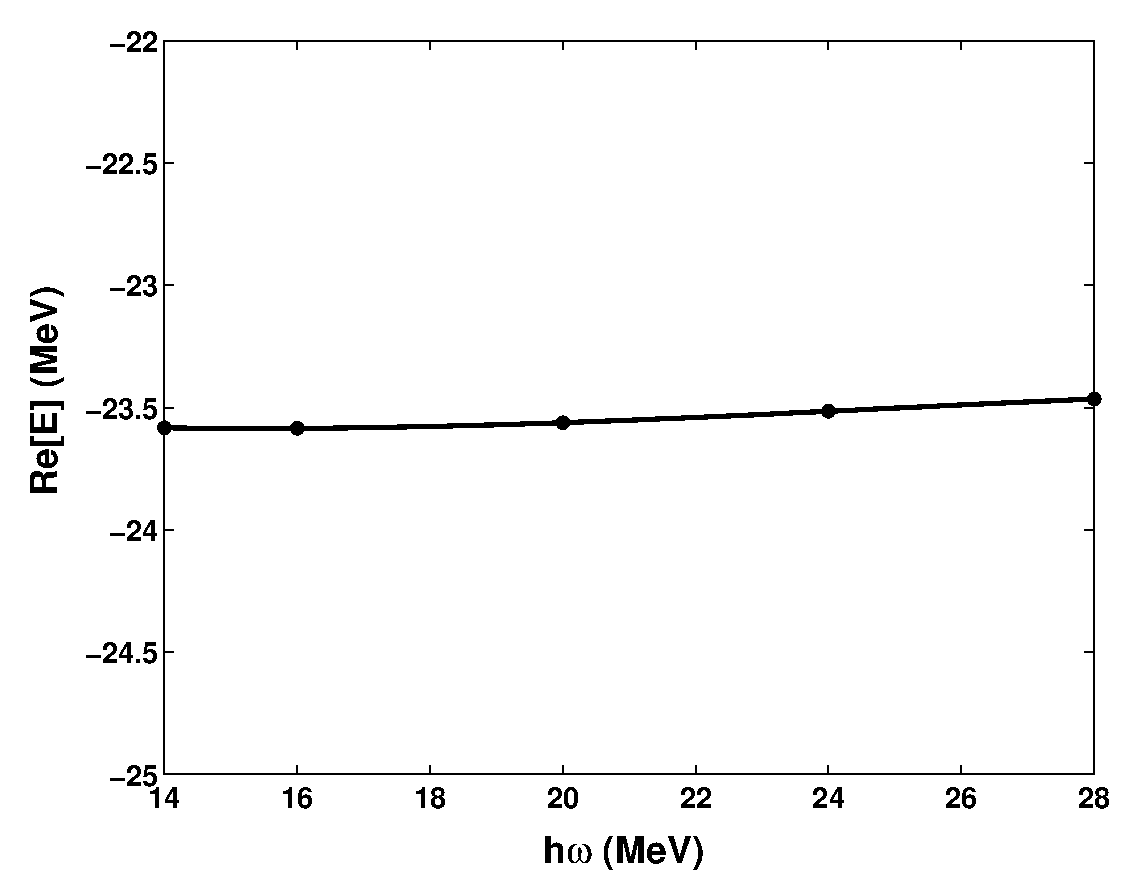
\epsfig{file=fig3.eps}}
  \caption{The $\hbar\omega$ dependence of the real part of the $^5$He ground state energy.} 
  \label{fig:he5_re_conv}
\end{figure}
\begin{figure}
  \resizebox{8cm}{5cm}{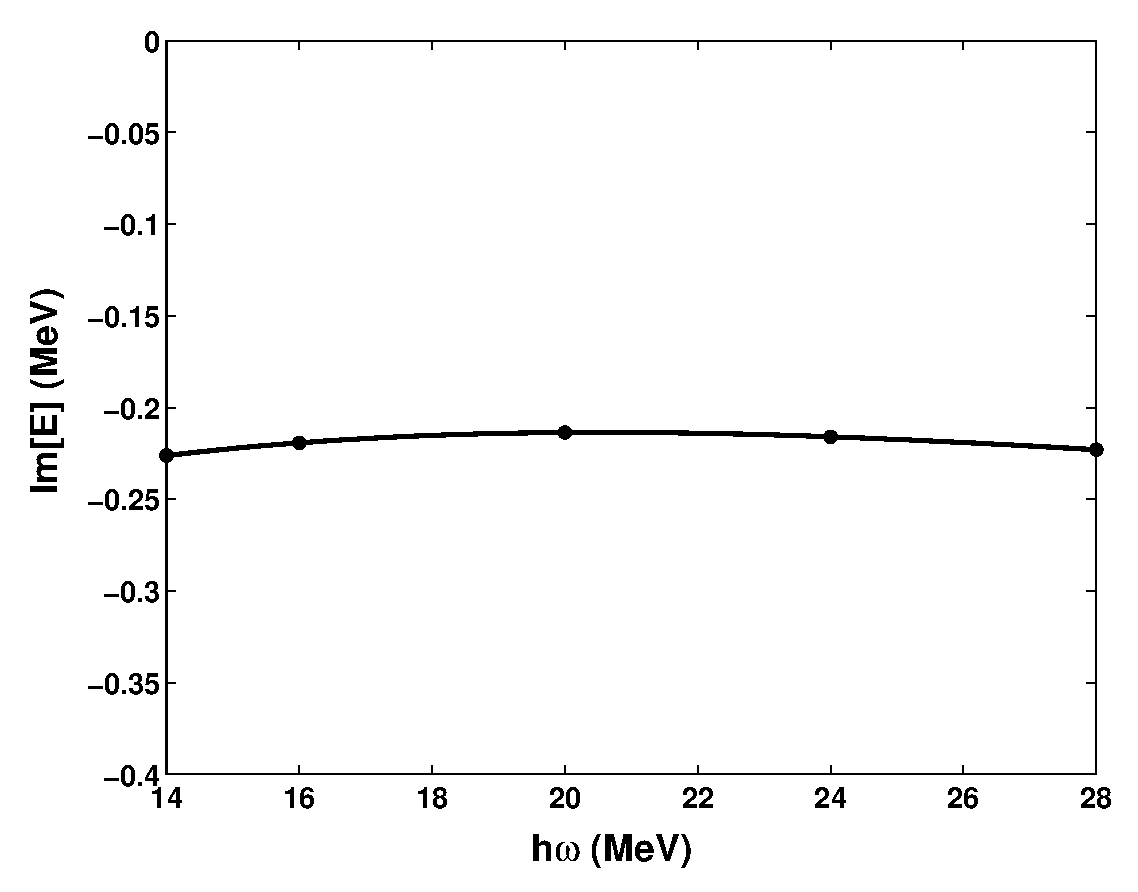
\epsfig{file=fig4.eps}}
  \caption{The $\hbar\omega$ dependence of the imaginary part of the $^5$He ground state energy.} 
  \label{fig:he5_im_conv}
\end{figure}
We observe that the 
dependence on $\hbar \omega�$ is very weak. For the real part 
it varies no more than 
$\sim100$~keV and for the imaginary part $\sim 10$~keV in range
of $\hbar \omega$  values. This is an indication 
that our basis is approximately complete, and
the error introduced through our basis truncation is smaller 
than the expected accuracy of the CCSD approximation.

Finally, we asses whether we have convergence with respect to the
number of discretization  points ($n = 20 $) of the countour $L_1^+$, 
definig our complex Woods-Saxon basis. We have already shown in the previous section 
that the Hartree-Fock energy for $^4$He is well converged 
with only $n=20$ points. In order to 
check whether the CCSD energy is converged we performed calculations of the $^5$He ground state
in the $s-d$ space using the two different contours given in Figs.\ref{fig:contour1} and \ref{fig:contour2}.
If our discretization of the contours is dense enough the two calculations should give exactly the 
same results for both the real- and imaginary parts of the energy.
In Figs.\ref{fig:he5_re_diffcont}  and \ref{fig:he5_im_diffcont} we give a plot 
of the convergence of the real and imaginary parts of the coupled cluster energy 
for the two different contours. It is seen that the real part of the CCSD energy differs by $10$keV and 
the imaginary part differs by only $\sim 3$keV, indicating that our results are well converged 
with respect to the number of integration points used to derive the Berggren basis for the $s-p$ neutron space.
\begin{figure}
\label{fig:he5_re_diffcont}  
\resizebox{8cm}{5cm}{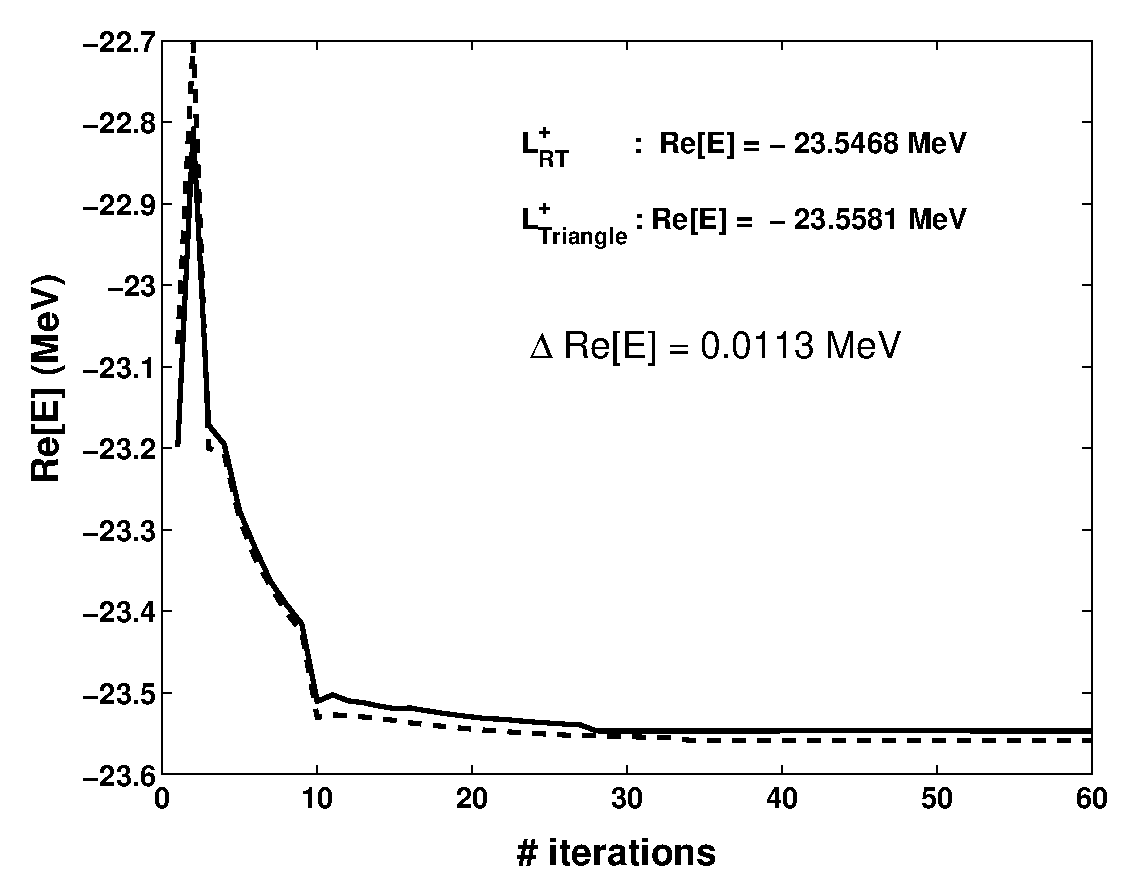
\epsfig{file=fig5.eps}}
  \caption{Convergence of the real part of the $^5$He ground state energy
    for two different contours $L^+$. The dashed line are 
    represents convergence with a triangular contour and the
    solid for a rotated+translated contour.}
  \end{figure}



\begin{figure}
  \resizebox{8cm}{5cm}{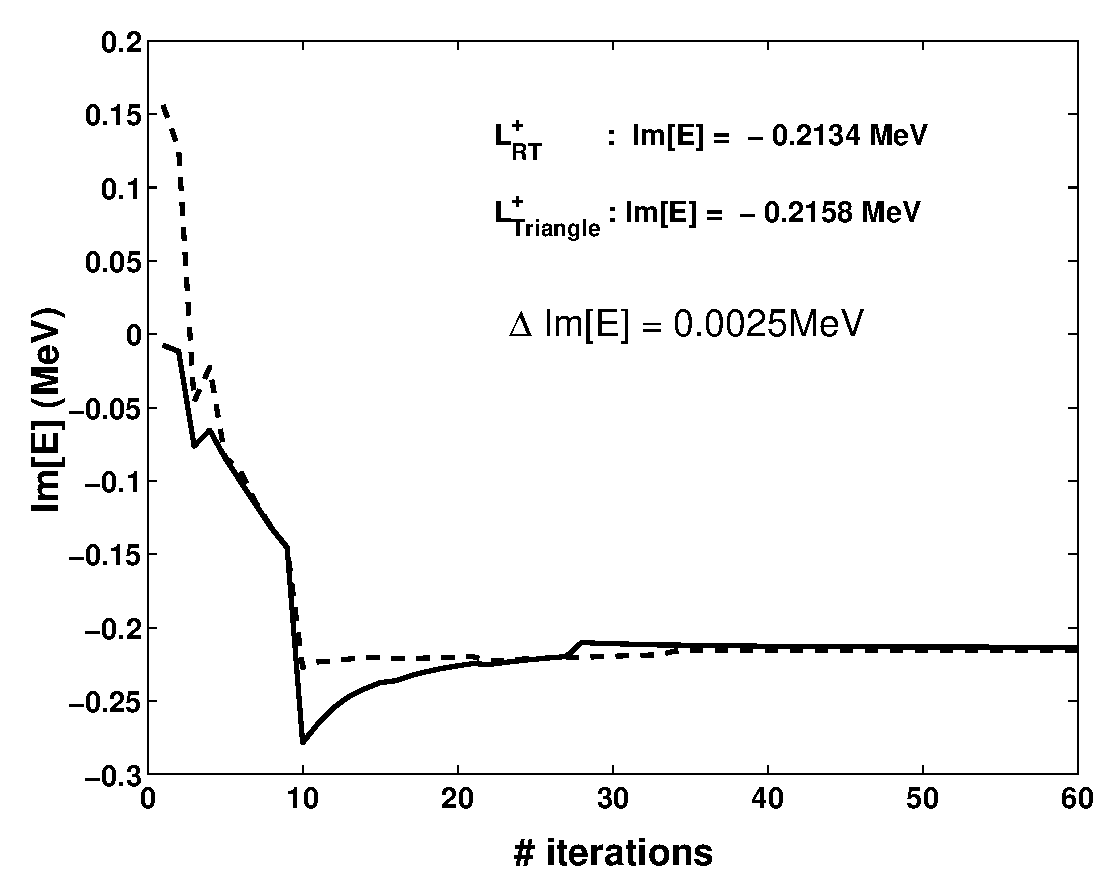
\epsfig{file=fig6.eps}}
  \caption{Same caption as in Fig.\ref{fig:he5_re_diffcont} 
    but for the imaginary part.}
  \label{fig:he5_im_diffcont}
\end{figure}


 

\section{Conclusion and future perspectives.}
\label{sec:conc}
We presented CCSD calculations of the $^{3-5}$He isotopes.  
Using a Gamow-Hartree-Fock basis, we depart
from Hermitian to non-Hermitian representations, and are therefore able to 
calculate resonant widths starting with the bare nucleon-nucleon interaction and
nucleon degrees of freedom. The calculated ground state energies of  
$^{3-4}$He are very close to the experimental values using 
a renormalized interaction of the low-momentum type ($V_{\mathrm{low-k}}$ derived from the 
N$^3$LO potential. For $^5$He ground state 
we are able to confirm that it is unstable with respect to one-neutron emission,
we get a width $\sim 0.35$MeV compared to the experimental value $\sim 0.65$MeV.
We have shown that single-reference CCSD is an accurate approximation for 
closed shell nuclei and nuclei with $\pm 1$ nucleon outside a closed shell ,by direct comparison 
with exact results in a small model-space.  
Convergence with respect to model-space size and discretization of the deformed contour $L^+$
defining our Berggren-basis has been checked, and we are quite confident that our results 
are well converged. 
Future work will involve implementation of triples corrections, three-body forces and study of matter
densities in loosely bound and unbound nuclei such as $^{11}$Li.

This work was supported in part by the U.S.~Department of Energy
under Contracts Nos.~DE-FG02-96ER40963 (University of Tennessee),
DE-FG05-87ER40361 (Joint Institute for Heavy Ion
Research), and the Research Council of Norway
(Supercomputing grant NN2977K). 
Oak Ridge National Laboratory is managed by UT-Battelle for the
U.S. Department of Energy under Contract No.~DE-AC05-00OR22725. 
Computational resources were provided by the National Energy
Research Scientific Computing Center (Berkeley) and the Leadership
Class Computing Facility (ORNL). 

\bibliography{library}

\end{document}
